\documentclass{article}

\usepackage[english]{babel}
\usepackage{microtype}
\usepackage{graphicx}
\usepackage{wrapfig}
\usepackage{enumitem}
\usepackage{fancyhdr}
\usepackage{amsmath}
\usepackage{chemformula}
\usepackage{index}
\usepackage{hyperref}
\usepackage[margin=1.0in]{geometry}
\usepackage{qtree}
\usepackage{float}
\usepackage{booktabs}
\usepackage{tabularx}
\usepackage{textcomp}

\begin{document}
\title{Summary: The Senses}
\author{Dowland Aiello}
\date{April 17, 2020}

\maketitle
\tableofcontents
\fancyhf{}

\newpage

\section{The function of sensory receptors in processing environmental data}

In order to respond to a particular stimulus, the body must first be capable of
capturing, interpreting, and applying data. The first of these three properties,
the capturing of data, is addressed through the utilization of \textbf{sensory
receptors}, which detect stimuli and, eventually, open or close an ion channel
in a neuron.

The process of \textbf{sensory transduction} describes the aforementioned
technique whereby sensory data is converted to a negative or positive
change in the charge of a neuron. For example, take the process whereby food
is digested:

\begin{enumerate}
	\item Sugar molecules bind to receptors in a taste receptor cell
	\item A signal transduction pathway is triggered, generating a
		\textbf{receptor potential} through a modification to the existent
		ion gradient
	\item The aformentioned ion gradient change, or signal, is propagated
		throughout the nervous system
	\item The signal reaches the brain, where it is processed, and conveyed as
		``perception.''
\end{enumerate}

As is the case with certain ``links'' between neurons (i.e., neuroplasticity),
this process is dulled through repeated activation, or \textbf{sensory
adaptation}.

\bigbreak{}

\begin{figure}[h]
	\centering
	\begin{minipage}{.5\textwidth}
		\centering
		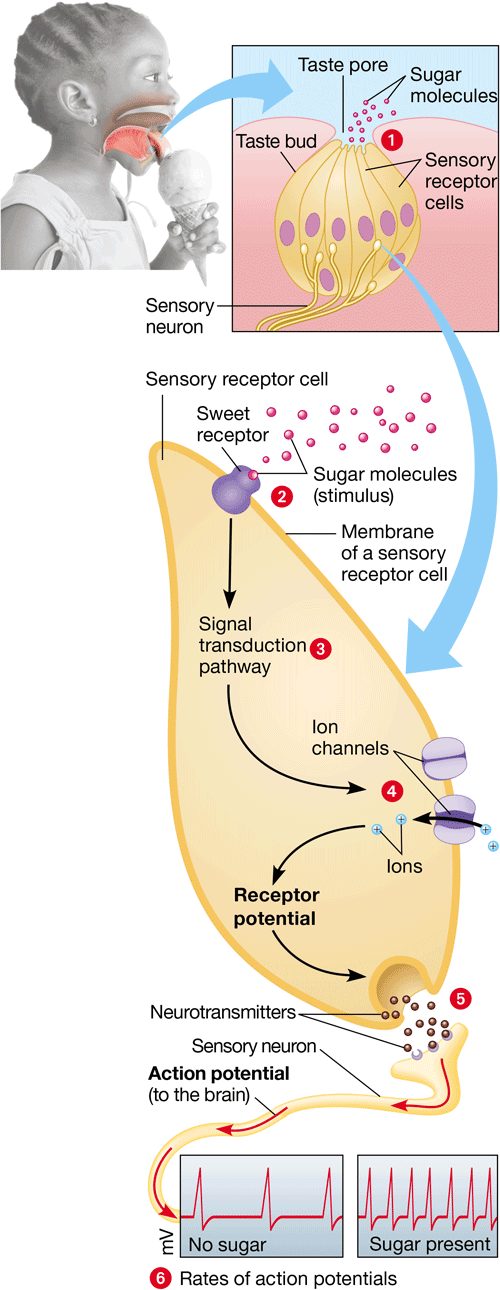
\includegraphics[height=\linewidth]{sugar_perception_a.png}
		\caption{Sensory transduction at a taste bud}
	\end{minipage}%
	\begin{minipage}{.5\textwidth}
		\centering
		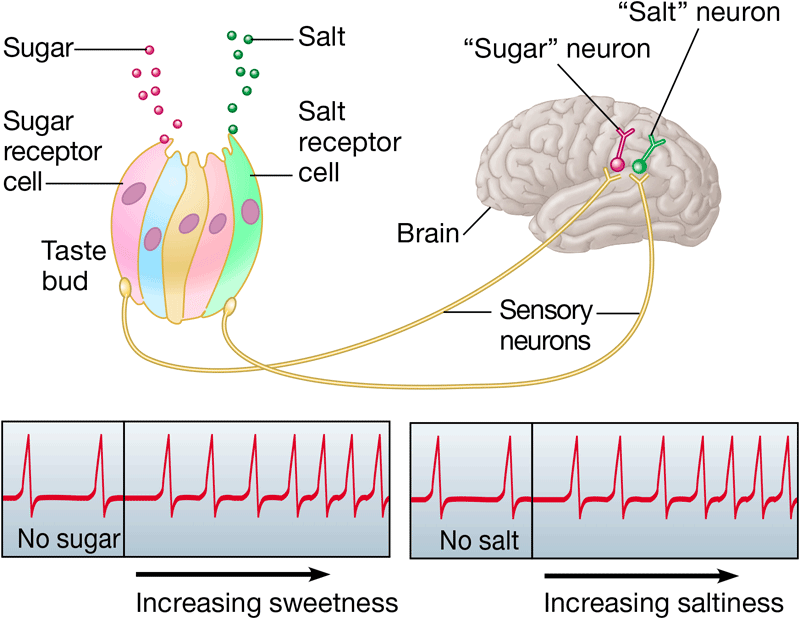
\includegraphics[width=\linewidth]{sugar_perception_b.png}
		\caption{Action potentials transmitting taste sensations}
	\end{minipage}
\end{figure}

\subsection{The various types of sensory receptors}

In animals, sensory cells are modeled to fit a specific class of stimuli.
Accordingly, sensory receptors are described with respect to the stimuli that
they ``match:''

\begin{enumerate}
	\item \textbf{Thermoreceptors}: detect heat or cold---exist in the skin,
		and deep in the body such that the receptors are capable of monitoring
		bloodstream temperature. Data received from these receptors are sent to
		the hypothalamus, which keeps the temperature of the body within a
		tolerable range.
	\item \textbf{Mechanoreceptors}: detect changes in environmental factors
		including pressure, touch, stretch, motion, or sound through manual
		stimulation by the environment (i.e., bending or stretching by
		environmental actors causes the plasma membrane to let more sodium or
		potassium in). Examples of mechanoreceptors in animals are:
		\begin{itemize}
			\item \textbf{Stretch receptors}: monitor the position of body parts
			\item \textbf{Hair cells}: detect sound waves and movement in fluid
		\end{itemize}
	\item \textbf{Pain receptors}: detect pain and minimize damage caused by
		intense presesure or temperature
	\item \textbf{Chemoreceptors}: detect chemical changes in the body or in
		the environment
	\item \textbf{Electromagnetic receptors}: detect electromagnetic energy
		(e.g., electricity, magnetism, light). A common example of an
		electromagnetic receptor found in animals is the \textbf{photoreceptor}
		---a receptor containing light-absorbing pigment
\end{enumerate}

\begin{figure}[h]
	\centering
	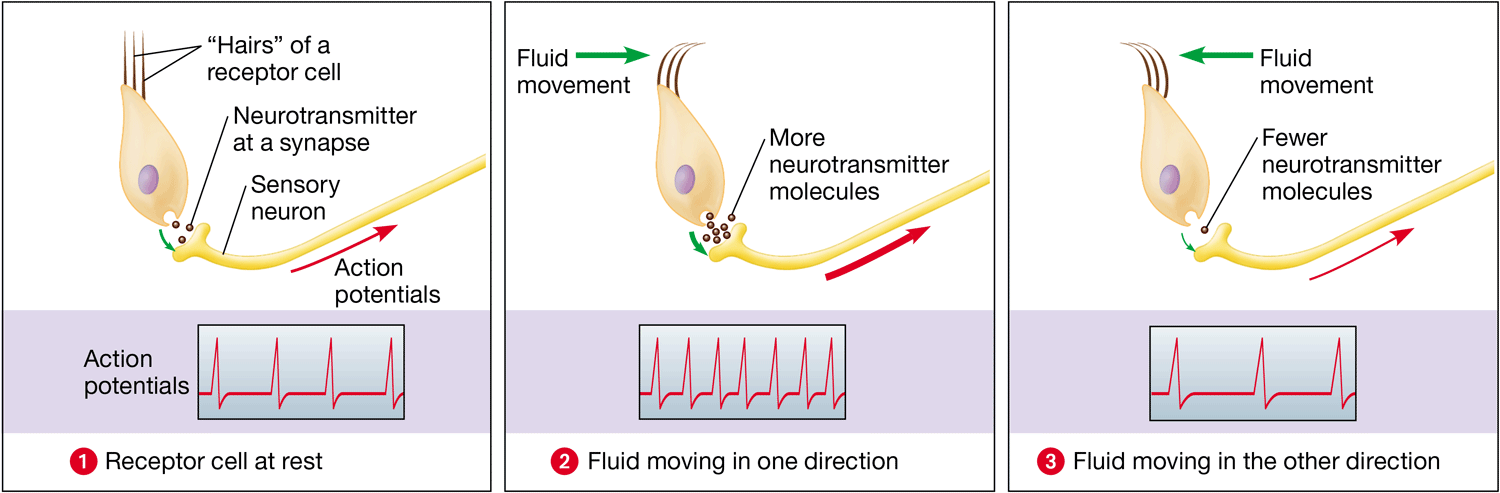
\includegraphics[width=0.9\linewidth]{hair_cell.png}
	\caption{Mechanoreception by a hair cell}
\end{figure}

\section{Hearing and balance}

\subsection{The structure of the ear}

In humans, the ear is instrumental to our innate sense of balance, and is
divided into three regions, each consisting of various components:

\begin{itemize}
	\item The \textbf{outer ear}, which is comprised by the:
		\begin{itemize}
			\item \textbf{Pinna}: the external part of the ear visible in daily
				life
			\item \textbf{Auditory canal}
		\end{itemize}
	\item The \textbf{middle ear}, which is separated from the outer ear by a
		sheet of tissue termed the \textbf{eardrum}, and is comprised by the:
		\begin{itemize}
			\item \textbf{Hammer} (malleus), \textbf{anvil} (incus), and
				\textbf{stirrup} (stapes), to which vibrations derived from sound
				pressure received by the eardrum are passed
			\item \textbf{Oval window}---vibrations conveyed through the
				stirrup, to which this structure is attached, pass through this
				hole in the skull bone, and into the inner ear
			\item \textbf{Eustachian tube}---through the connective capability
				provided by this structure, air pressure parity is maintained
				between the inner ear and the pharynx
		\end{itemize}
	\item The \textbf{inner ear}, which is comprised by the following fluid-
		filled chambres:
		\begin{itemize}
			\item \textbf{Cochlea}: consists of the
				\begin{itemize}
					\item \textbf{Organ of Corti}---the human hearing organ
						composed of various \textbf{basilar membrane}-embedded
						hair cells
				\end{itemize}
		\end{itemize}
\end{itemize}

\begin{figure}[h]
	\centering
	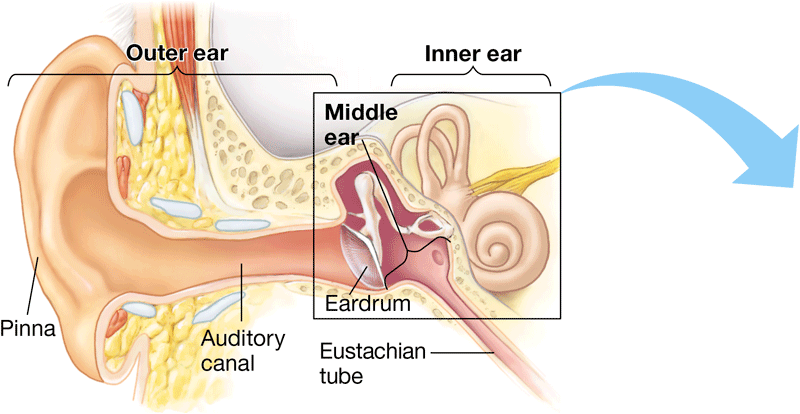
\includegraphics[width=0.8\linewidth]{ear_structure.png}
	\caption{The structure of the human ear}
\end{figure}

\subsection{The ear as an organ of balance}

In addition to each of the aforementioned functions, the ear aids in the
perception of position, movement, and balance, through the utilization of
several structures located adjacent to the cochlea named the
\textbf{semicircular canals}, which deal specifically with detecting
changes in angular movement and rate of rotation. Each of these canals
operate on the basis of the movement of a \textbf{capula}, or a thick,
sticky fluid against which hairs in the canal are placed. Higher rates of
movement result in faster movement of the capula, resulting in a greater
frequency of released action potential signals from this organ.

\section{Vision}

In invertebrates, \textbf{compound eyes} are the image-forming sensory organs
of the body. These functional groupings of components contain thousands of
light-detecting \textbf{ommatidia}, which capture a ``field of view'' of light.
Each of these parallel stream of information contributes to a larger picture,
which is splied together by the brain of the animal.

In all vertebrates, \textbf{single-lens eyes} are the image-forming sensory organs
of the body. Though it is more structurally complicated than the compoudn eye, the
single-lens eye can be broken down into various functional groups. For example,
as is often useful in studying the ear, the eye can be divided into a front and
rear chamber---both of which are filled with fluid. These fluids---the aqueous
and more viscous vitreous humors, respectively---aid in the circulation of
necessary minerals and nutrients, and dispose of waste. With a more practical
focus towards the functionality of the single-lens eye, one might turn to the
following structures:

\begin{itemize}
	\item The \textbf{cornea}: helps let light into and focus the eye
	\item The \textbf{choroid}: composed of the
		\begin{itemize}
			\item \textbf{Iris}: allows more or less light into the eye by
				modifying its diameter
			\item \textbf{Pupil}: receives and transfers light to a lens
		\end{itemize}
	\item A \textbf{lens}: conveys light in a focused manner\footnote{generally,
			an eye is focused through a process of accomodation,
			wherein ciliary muscles are contracted or relaxed and ligaments are
			loosened or tightened.
		}onto the
		\textbf{retina}, and its constituent photoreceptors\footnote{in humans,
			there are two types of photoreceptors: \textbf{rods}, which are more
			sensitive to light, and \textbf{cones} which are more suited for
			color. These types of photoreceptors each contain their respective
			pigments which account for their abilities to discern different types
			of incoming light (i.e., \textbf{rhodopsin} in rods and
			\textbf{photopsins} in cones).
		}---of which there are
		the most of towards the \textbf{fovea} or center of the eye
\end{itemize}

\begin{figure}[h]
	\begin{minipage}{.5\textwidth}
		\centering
		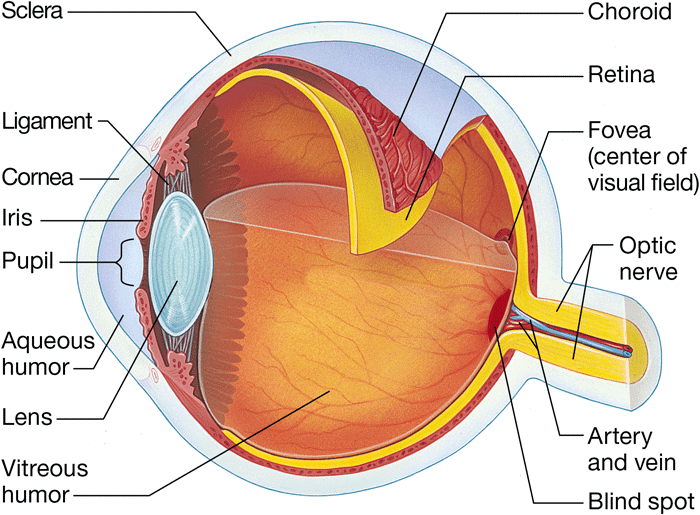
\includegraphics[width=0.82\linewidth]{single_lens_eye.png}
		\caption{The single-lens eye of a vertebrate}
	\end{minipage}%
	\begin{minipage}{.5\textwidth}
		\centering
		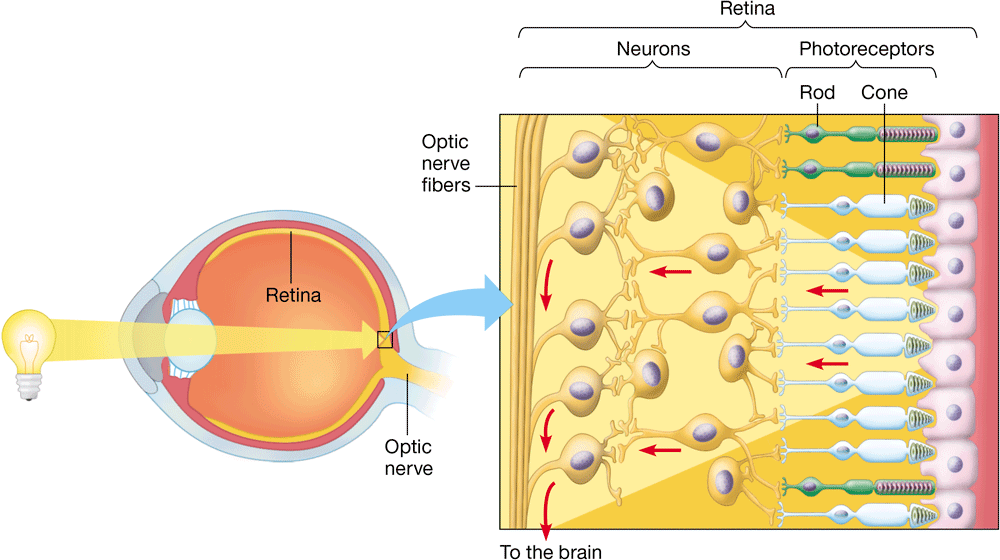
\includegraphics[width=\linewidth]{single_lens_eye_rods_cones.png}
		\caption{The transfer of light data through the eye}
	\end{minipage}
\end{figure}

\section{Taste and Smell}

In the nasal cavity, \textbf{olfactory} receptors are responsible for informing
the portion of the brain responsible for the sensation of smell (i.e., the
olfactory bulb) of incoming stimulus data. This is achieved through the binding
of an odorous sustance to receptor proteins in nasal cilia.

In the mouth, responsibilities for certain tastes are deleagted to specific
taste buds on the tongue. Namely, umami, swwet, sour, salty, and bitter are each
detected by only one kind of taste receptor.

\end{document}
